\section{Задание №9}

Рассмотреть два вида процессов:
\begin{itemize}
        \item Винеровский процесс $W(t)$, $t \in [0,\,1]$, $W(0) = 0$.
        \item Процесс Орнштейна--Уленбека $X(t)$, $t \in [0,\,1]$, $X(0) = X_0$, то есть стационарный гауссовский процесс. Начальные значения $X_0$ генерируются случайным образом так, чтобы получееный процесс был стационарным.
\end{itemize}
Для данных гауссовских процессов:
\begin{enumerate}
        \item Найти ковариационную функцию и переходные вероятности;
        \item Моделировать независимые траектории процесса с данными переходными вероятностями методом добавления разбиения отрезка;
        \item Построить график траектории, не соединяя их ломанной, с целью получения визуально непрерывной линии.
\end{enumerate}


\subsection{Винеровский процесс}

\begin{definition}
        Рассмотрим вероятностное пространство $(\Omega,\,\mathcal{F},\,\p)$. Тогда назовём \textit{случайным процесом} параметризированное семейство $\{\,W_t\,\}_{t \in T}$ случайных величин 
$$
        W_t:\Omega\to\R,\;t\in T,\;T \subset [0,\,+\infty).
$$
        В данном случае мночество параметров интерпретируется как некоторый временной интервал.
\end{definition}

\begin{definition}
        Будем называть случайный процесс $\{\,W_t\,\}_{t\in T}$ \textit{гауссовским}, если для любых $t_0,\,t_1,\,\ldots,\,t_n\in T$ соответствующий случайный вектор $w = (W_{t_1},\,W_{t_2},\,\ldots,\,W_{t_n})$ имеет многомерное нормальное распределение, то есть имеет плотность
$$
        \rho(W_{t_1},\,\ldots,\,W_{t_n})
=
        \frac{1}{(2\pi)^{\nicefrac{n}{2}}|R|^{\nicefrac{1}{2}}}
\cdot
        \exp\left\{
-\frac{1}{2} \cdot
\langle\, R^{-1}(w - m),\, w - m\,\rangle
        \right\},
$$
        где $m = (m_1,\,m_2,\,\ldots,\,m_n)^\T$~--- вектор средних, а $R \in \R^{n \times n}$~--- ковариационная матрица: $R = \|\mbox{cov}(t_i,\,t_j)\|_{i,\,j}$, $R = R^\T > 0$.
\end{definition}

\begin{definition}
        Определим \textit{винеровский процесс} как гауссовский процесс на отрезке $[0,\,1]$ с нулевым средним и ковариационной функцией $\mbox{cov}(W(t_i),\,W(t_j)) = \min\{t_i,\,t_j\}$.
\end{definition}

Выпишем основные свойства этого процесса. Доказательство этих свойств можно найти у Ширяева. Итак:
\begin{enumerate}
        \item $W(0) = 0$ почти наверное;
        \item $W(t)$ является непрерывной функцией (по переменной $t$);
        \item Приращения функции $W(t)$ независимы и имеют стандартное нормальное распределение, то есть $W(t_2) - W(t_1) \sim \mbox{N}(0,\,1)$, для любых $t_1 < t_2$.
\end{enumerate}

\subsubsection{Переходные вероятности}

Рассмотрим отрезок~$[t_1,\,t_2] \subset T$ и его внутреннюю точку $t = t_1 + \alpha(t_2 - t_1)$, $0 < \alpha < 1$. И найдем условную плотность
$$
        \rho_{W(t)}(x\,|\,W(t_1) = x_1,\, W(t_2) = x_2)
=
        \frac{
\rho_{W(t_1),\,W(t),\,W(t_2)}(x_1,\,x,\,x_2)
        }{
\rho_{W(t_1),\,W(t_2)}(x_1,\,x_2).
        }
$$
Обозначим векторы $\hat x = [x_1,\,x_2]^\T$ и $\hat{\hat x} = [x_1,\,x,\,x_2]^\T$. Тогда плотности вероятностей равны
$$
        \rho_{W(t_1),\,W(t_2)}(\hat x)
=
        \frac{1}{2\pi\sqrt{|R_2|}}\cdot \exp\left\{-\frac12 \hat x^\T R_2^{-1} \hat x\right\},
$$
$$
        \rho_{W(t_1),\,W(t),\,W(t_2)}(\hat{\hat x}) = \frac{1}{(2\pi)^{\nicefrac{3}{2}}\sqrt{|R_3|}}\cdot\exp\left\{\frac12 \hat{\hat x}^\T R_3^{-1}\hat{\hat x}\right\}.
$$
Здесь за $R_2$ и $R_3$ обозначены соответствующие ковариационные матрицы:
$$
        R_2 = \begin{pmatrix}
        t_1 & t_1 \\
        t_1 & t_2
        \end{pmatrix},
        \qquad
        R_3 = \begin{pmatrix}
                t_1 & t_1 & t_1 \\
                t_1 & t   & t   \\
                t_1 & t   & t_2
        \end{pmatrix}
        .
$$
Теперь посчитаем определители и обратные ковариационных матриц:
$$
        |R_2|
=
        t_1
        (t_2 - t_1),
\qquad
        |R_3|
=
        t_1
        (t - t_1)
        (t_2 - t).
$$
$$
        R_2^{-1}
=
        \begin{pmatrix}
\frac
  {t_2}
  {t_1
   (t_2 - t_1)}
        &
-
\frac
  {1}
  {t_2 - t_1}
        \\
-
\frac
  {1}
  {t_2 - t_1}
        &
\;\;\;
\frac
  {1}
  {t_2 - t_1}
        \end{pmatrix}
$$
$$
        R_2^{-1}
=
        \begin{pmatrix}
\frac
  {t}
  {t_1
   (t - t_1)}
        &
-
\frac
  {1}
  {t - t_1}
        &
0
        \\
-
\frac
  {1}
  {t - t_1}
        &
\frac
  {t_2 - t_1}
  {(t_2 - t)
   (t - t_1)}
        &
-
\frac
  {1}
  {t_2 - t}
        \\
0
        &
-
\frac
  {1}
  {t_2 - t}
        &
\;\;\;
\frac
  {1}
  {t_2 - t}
        \end{pmatrix}  
$$
Соединим все вместе и получим
$$
        \rho_{W(t)}
        (
          x
          \;|\;
          W(t_1) = x_1
          ,\,
          W(t_2) = x_2
        )
=
        \frac
          {
            1
          }
          {
            \sqrt{
              2
              \pi
              (1 - \alpha)
              (t_2 - t_1)
            }
          }
        \exp
        \left\{
          -
          \frac
          {
            (
              x
              -
              (1 - \alpha) x_1
              +
              \alpha x_2
            )^2
          }
          {
            2
            \alpha
            (1 - \alpha)
            (t_2 - t_1)
          }
        \right\}.
$$


\subsubsection{Алгоритм}
        \begin{enumerate}
                \item
Сначала определим значения винеровского процесса на концах отрезка $[0,1]$. По условию $t_0 = 0$, $W(t_0) = 0$, $t_1 = 1$. Величину $W(t_1)$ разыграем как $\mathrm{N}(0,\,1)$.
        \item
Будем рекурсивно делить отрезки $[t_0, t_1]$ в некотором отношении $\alpha$. Затем считать значение случайной величины $W(t)$ по выведенной формуле условной плотности. Это просто, если заметить тот факт, что:
$$
        W(t)
\sim
        \mathrm{N}
        (
          (1 - \alpha)
          x_1
          +
          \alpha
          x_2
        ,\,
          \alpha
          (1 - \alpha)
          (t_2 - t_1)
        ).
$$
        \item
Остановим алгоритм по достижении заданной точности $t_{k+1} - t_k < \varepsilon$.
\end{enumerate}
\begin{remark}
        Проверить правильность вычислений можно дополнительно построив доверительный интервал. В нашем случае можно воспользоваться правилом трех сигм.
\end{remark}





\clearpage
\begin{figure}[t]
        \noindent
        \centering
        {
                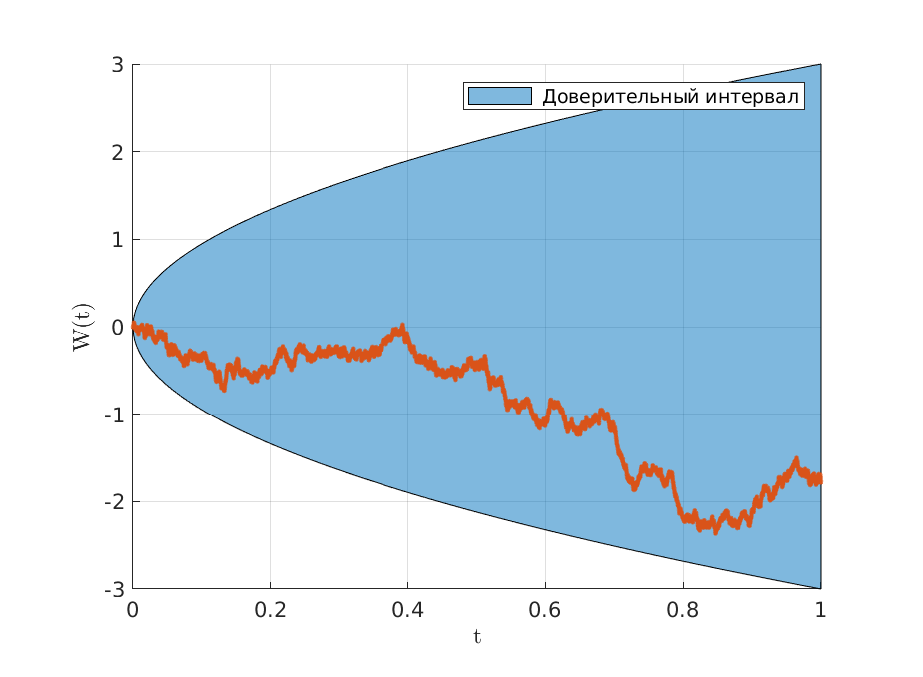
\includegraphics[width=120mm]{task_09/weiner.eps}
        }
        \caption{Поточечный график винеровского процесса демонстрирует его непрерывность. Параметрами алгоритма были взяты $\alpha = 0,\!3$, $\varepsilon = 10^{-4}$.}
\end{figure}
\begin{figure}[b]
        \noindent
        \centering
        {
                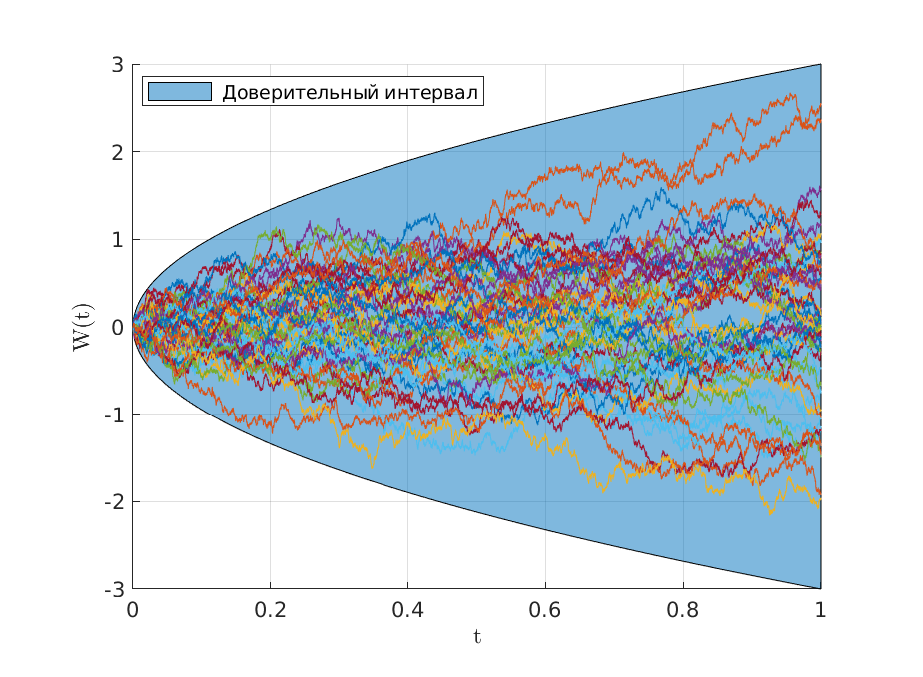
\includegraphics[width=120mm]{task_09/50-weiners.eps}
        }
        \caption{Представлены 50 винеровских процессов.}
\end{figure}
\clearpage


\subsection{Процесс Орнштейна--Уленбека}

\begin{definition}
        Случайный процесс $\{W_t\}_{t\in T}$ называется \textit{стационарным}, если конечномерные распределения инвариантны относительно сдвига времени.
\end{definition}

\begin{definition}
        Гауссовский процесс $\{W_t\}_{t\in T}$ называется \textit{процессом Орнштейна--Уленбека}, если он является стационарным и марковским.
\end{definition}

Из-за того, что процесс Орнштейна--Уленбека является стационарным, он обладает следующими свойствами:
$$
        \E\,W(t) = \mu = \mathrm{const},
\qquad
        R(t, s) = R(|s - t|).
$$
Не ограничивая общностей, будем рассматривать процесс при $\mu = 0$. Введем обозначение $\Var\,W(t) = \sigma^2$. Тогда
$$
        R(t, s) = \sigma^2 \rho(s,t),
\quad
        \mbox{где } \rho(s,t)\mbox{ коэффициент корреляции.}
$$

\begin{theorem}
        Для того, чтобы последовательность $W_1, \ldots, W_n$ нормально распределенных случайны величин была марковской, необходимо и достаточно, чтобы
$$
        \rho(j,k) 
        = 
        \rho(j, i)
        \cdot
        \rho(i, k),
        \quad
        \forall i,j,k
        \,:\,
        j \leqslant i
        < k \leqslant n,
$$
где $\rho(i,j)$ --- коэффициент корреляции случайных величин $W_i$ и $W_j$.
\end{theorem}

В силу того, что процесс $W(t)$ является марковским, то
$
        \rho(s,t)
        =
        \rho(s,\tau)
        \cdot
        \rho(\tau, t)
$.
В силу же того, что $R(s,t) = R(|s - t|)$, то $\rho(s,t) = \rho(s - t)$.
Тогда введем замену переменных:
$
        x = s - \tau
$,
$
        y = \tau - t
$.
Получим, что
$$
        \rho(x + y)
        =
        \rho(x)
        \cdot
        \rho(y).
$$

\begin{theorem}
        Пусть функция $f(t)$ определена при $t > 0$ и ограничена на каждом конечном интервале. Если $f(t)$ удовлетворяет соотношению $f(t + s)$ = $f(t)f(s)$, то или $f(t) \equiv 0$, или $f(t) = e^{-\lambda t}$, где $\lambda$ --- некоторая положительная константа.
\end{theorem}

Получается, что задача распадается на два варианта: когда $\rho(t) \equiv 0$ и иначе. Первый случай равносилен тому, что ковариационная функция $\mathrm{cov} (W(t),W(s))$ также равна нулю. Это значит, что случайные величины $W(t)$ независимы в совокупности. Поэтому будем моделировать каждую случайную величину как $\mathrm{N}(\mu, \sigma^2)$.

Теперь рассмотрим случай $\rho(s, t) = e^{-\lambda|s - t|}$, $\lambda > 0$. Тогда ковариационная функция рассматриваемого процесса имеет вид $R(s,t) = \sigma^2 e^{-\lambda|s-t|}$. Найдем переходную плотность:
$$
        \rho_{W(t)}(x_1\,|\,W(s) = x_2)
=
        \frac
          {\rho_{W(t),W(s)}(x_1,x_2)}
          {\rho_{W(s)}(x_2)}.
$$
Мы можем выписать формулу для каждой из плотностей, участвующих в выражении, так как рассматривается гауссовский процесс:
$$
        \rho_{W(t),W(s)}(x_1,x_2)
=
        \frac
          {1}
          {2
           \pi
           |C|^{\nicefrac12}
          }
        \exp
        \left\{
          -
          \frac12
          \langle
            x,\,C^{-1}x
          \rangle
        \right\},
\quad
        \mbox{где }
        x = (x_1,\,x_2)^\T.
$$
$$
        \rho_{W(s)}(x_2)
=
        \frac
          {1}
          {
            \sqrt{2\pi}
            \sigma
          }
        \exp
        \left\{
          -
          \frac
           {
             x_2^2
           }
           {
             2\sigma^2
           }
        \right\}.
$$
Здесь $C$ --- ковариационная матрица. Запишем ее, ее определитель и обратную:
$$
        C
=
        \begin{pmatrix}
\sigma^2 & R(t,s)   \\
R(t,s)   & \sigma^2
        \end{pmatrix},
\quad
        |C|
=
        \sigma^4
        -
        R^2(t,s),
\quad
        C^{-1}
=
        \frac{1}{|C|}
        \begin{pmatrix}
\sigma^2 & -R(t,s)  \\
-R(t,s)  & \sigma^2
        \end{pmatrix}.
$$
Соберем все вместе:
$$
        \rho_{W(t)}(x_1\,|\,W(s) = x_2)
=
        \frac{1}
        {
\left(
  2\pi
  \left(
    \sigma^2
    -
    \frac{R^(t,s)}{\sigma^2}
  \right)
\right)^{\nicefrac{1}{2}}
        }
        \exp
        \left\{
-
\frac
{
        \left(
          x_1
          -
          \frac{R(t,s)}{\sigma^2}
          x_2
        \right)^2
}
{
        2
        \left(
          \sigma^2
          -
          \frac{R^2(t,s)}{\sigma^2}
        \right)
}
        \right\}.
$$

\subsubsection{Алгоритм}
